% !TEX root = ../thesis.tex

\chapter{Neural network triggers}
\label{chap:neural-network-triggers}

% \todo{write introductory shit here?}

\section{Motivation}
\label{sec:motivation}

The station-level triggers in the previous chapter have been shown to perform well for the science case of the Pierre Auger Observatory. However, it has 
also been concluded that a lot of potential data, especially at low energies is ignored. This is by intention in order to keep DAQ readout at feasible levels.

Attempts at improving the overal efficiency of the SD triggers can be made. This is only possible to a certain level. At lowest energies the particle cascade is 
not big enough to warrant coincident triggers in at least 3 WCD stations. As per \autoref{sssec:bayesian-folding}, the lateral trigger probability a given 
classification algorithm can maximally achieve is given by the LPP (c.f. \autoref{fig:fitfunction-comparison}). The T3 detection probability of such an ideal 
trigger, and consequently the maximal efficiency for an array with $\SI{1.5}{\kilo\meter}$ spacing is compared to the efficiency of classical triggers in 
\autoref{fig:ideal-efficiency-comparison}.

Of course, efficiency can be improved simply by adjusting trigger thresholds of the algorithms in \autoref{sec:trigger-implementation}. However, the more lenient
these thresholds are, the more background events will be detected. This quickly results in trigger rates that are unmanagable for the infrastructure at the Pierre 
Auger observatory. The probability with which time traces correctly raise a T2 is shown alongside the resulting random-trace trigger rate for different thresholds
of classical algorithms in \autoref{fig:classical-trigger-roc}.

Ideally, neural network architectures developed in this chapter should undercut the random-trace trigger rate of classical triggers, while retaining an overall 
higher accuracy. That is, they lay below and right of the operating point in \autoref{fig:classical-trigger-roc}. For any algorithm that achieves this, the 
corresponding LTP will be greater than that of classical triggers, resulting in higher event detection efficiency, while not exceeding the bandwidth limitations 
of the underlaying hardware. 

\begin{figure}
	\begin{subfigure}[b]{0.49\textwidth}
		\centering
		\includegraphics[width=\textwidth]{./plots/ideal_t3_efficiency.png}
		\caption{\textbf{T3 efficiency}}
		\label{fig:ideal-efficiency-comparison}
	\end{subfigure}
	\hfill
	\begin{subfigure}[b]{0.49\textwidth}
		\centering
		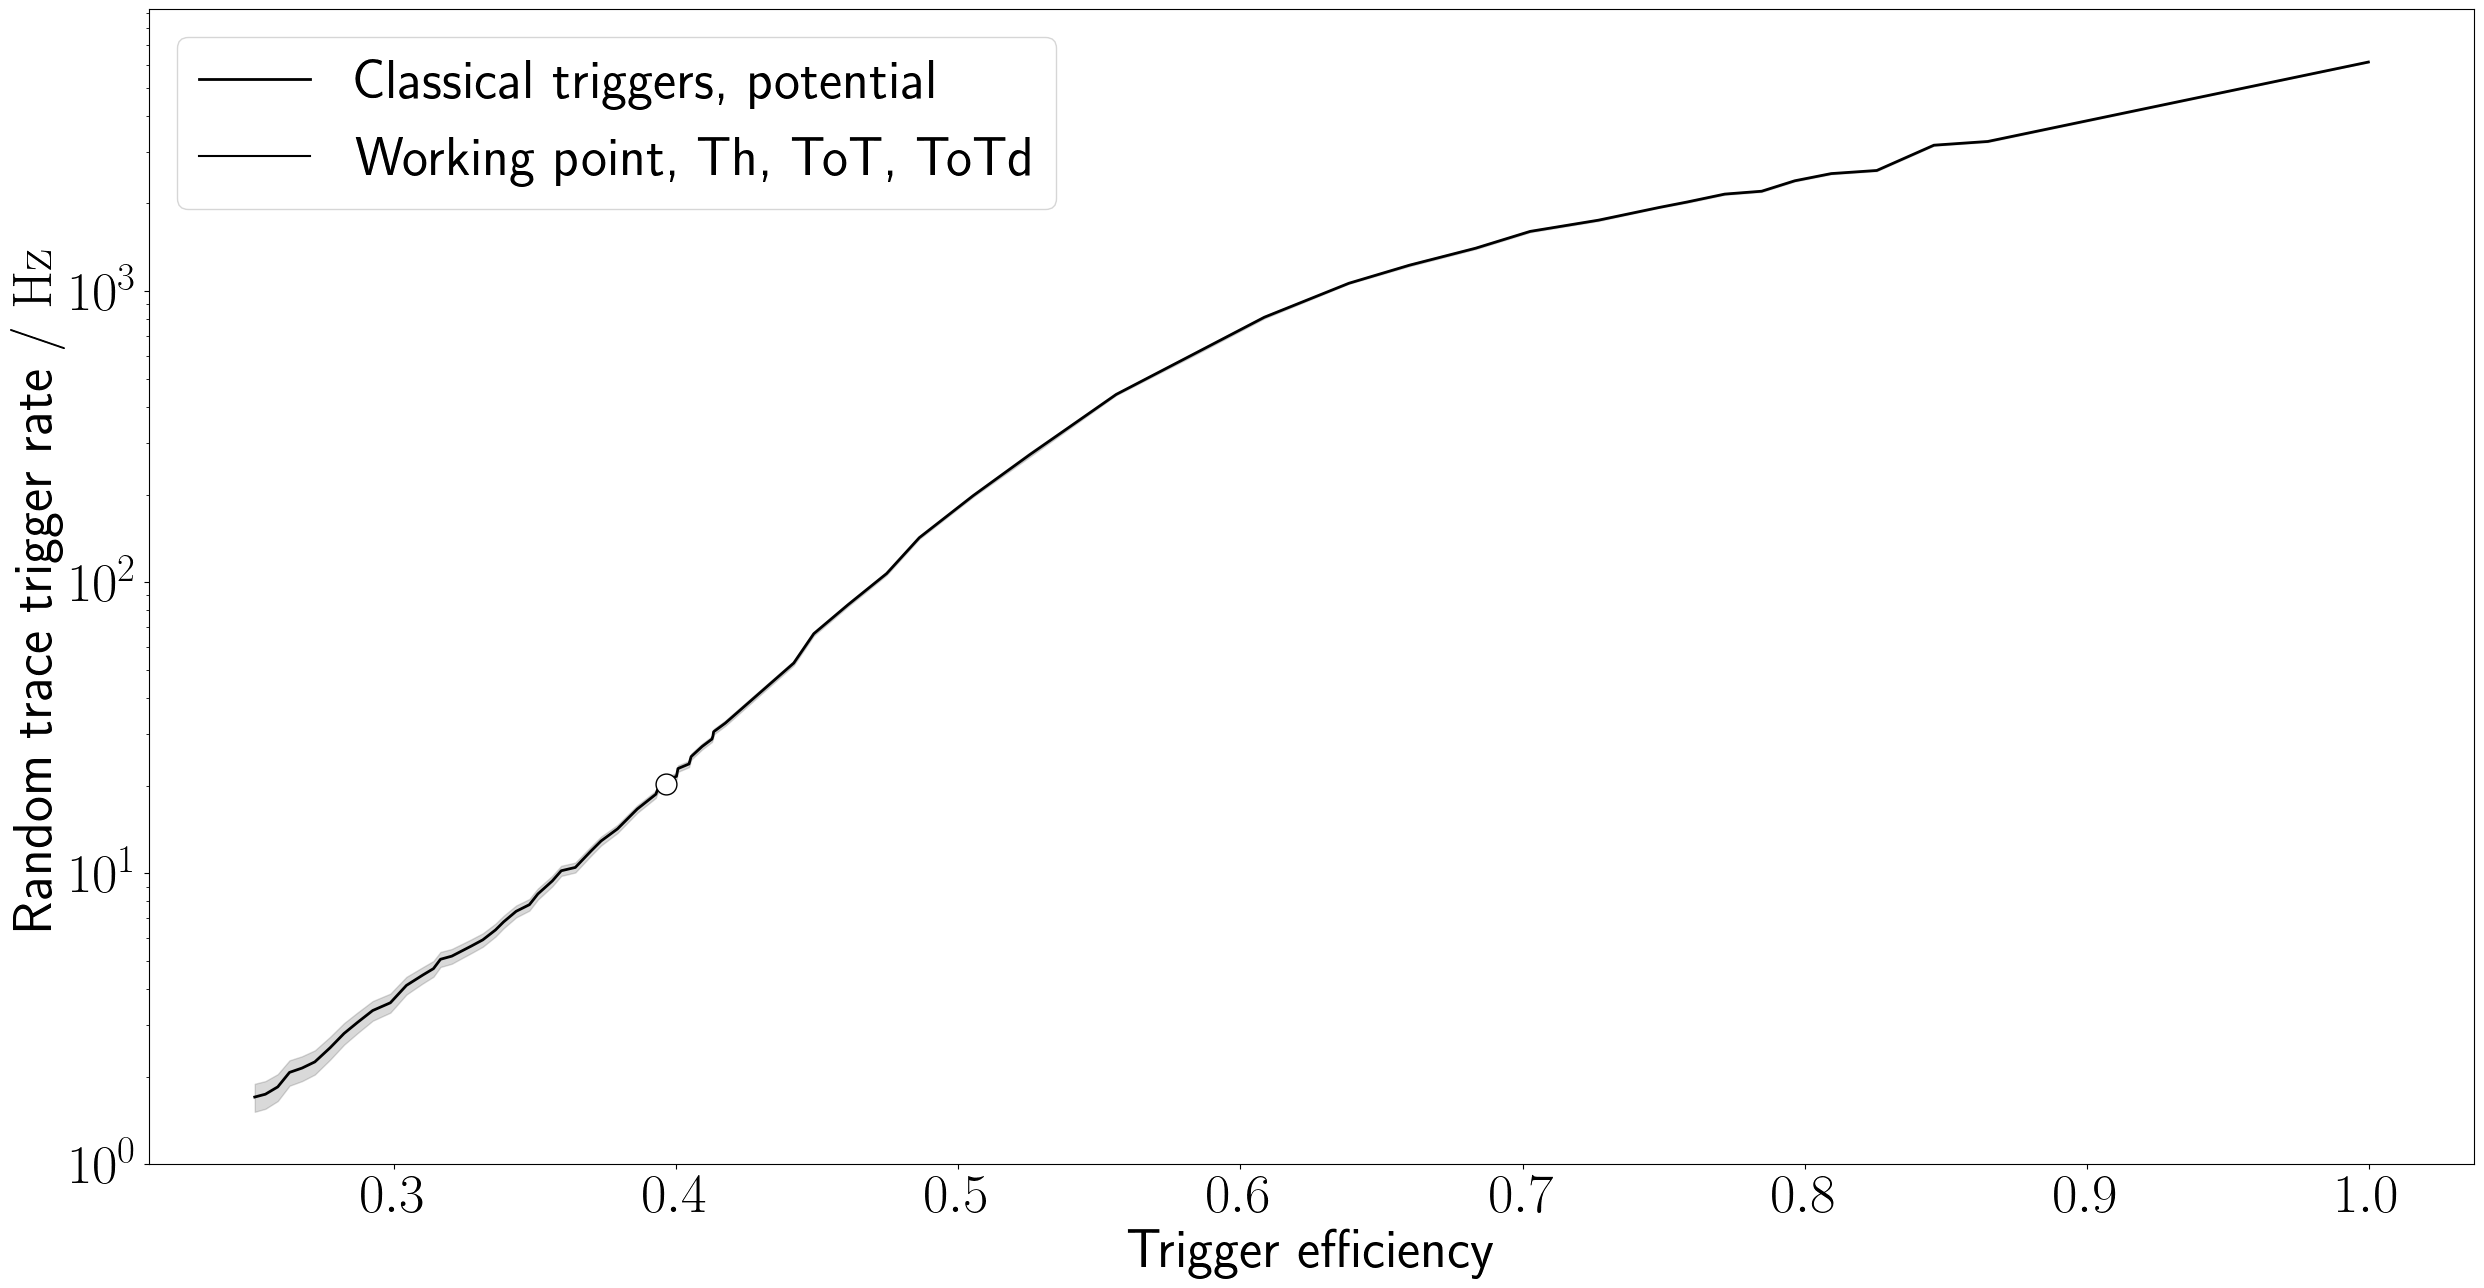
\includegraphics[width=\textwidth]{./plots/classical_trigger_ROC.png}
		\caption{\textbf{Classical trigger potential}}
		\label{fig:classical-trigger-roc}
	\end{subfigure}
	\caption{\textbf{(a)} Comparison of an ideal trigger sensitive to any shower signal from primary energies $E\geq\SI{10}{\peta\electronvolt}$ to classical 
    triggers. \textbf{(b)} The noise level over calculated efficiency for classical triggers. The tail ends of the potential curve are calculated by adjusting the
    trigger thresholds from $+250\%$ to $-95\%$ of the nominal values.}
\end{figure}

\section{Implementation}
\label{sec:implementation}

The python library TensorFlow \cite{tensorflow2015-whitepaper} is used as a backend to implement the individual classifiers. All discussed architectures are built 
and trained with the release version 2.8.4 \cite{tensorflowversion}. Adjustments to the trainable parameters are calculated according to a momentum-based 
stochastic gradient descent (Adam \cite{kingma2014adam}) on a batch level. In this context, a single batch is made up of all traces that are recorded from a single 
air shower event. Since batch size grows quickly with increasing energy, a generative approach, where traces are created (c.f. \autoref{sec:trace-building}) at 
runtime upon requirement, is used in building training data in order to make the process as RAM-efficient as possible. This has important implications. As trace 
building relies heavily on randomization, the actual training data will not be the same if the random number generators are not seeded beforehand. This has been
taken into account. All networks are - unless specifically stated otherwise - trained and validated using the same signal input data.

\section{Design consideration}
\label{sec:design-considerations}

\subsection{Architecture}
\label{ssec:architecture}

The hardware specifications at the FPGA level, where trigger conditions are currently checked, are limited. For this reason, NN architectures should be kept as 
simple as possible. Most importantly, the number of weights, biases and other trainable parameters will need to be hardcoded into station software. Because of 
minimal available storage space, this number needs to be kept low.

This immediately disqualifies powerful candidates like autoencoders or transformers (compare \autoref{sec:NN-other}) from consideration. Only  relatively simple 
dense-, convolutional-, or recurrent neural network architectures are viable contenders and might be implementable in the SD electronics.

\subsection{Choice of input data}
\label{ssec:input-data}

As stated in the previous chapters, neural networks learn by example. It is imperative that the input data propagating through the network during training 
resembles later use-case inputs as much as possible. However, some choices in how data is represented can and need to be made in order to benefit loss 
minimization. 

\subsubsection{Prior probability}
\label{sssec:prior-discussion}

The flux of cosmic rays with energies exceeding the proton knee is tiny ($\mathcal{O}(\SI[per-mode=power]{1}{\per\meter\per\year})$ \cite{dembinski2017data}). 
While the size of the SD guarantees decent exposure over the entire array, an individual station will mostly measure background. In fact, the prior probability $p$
of encountering events beyond the kee in a random time trace is roughly one in one million. Of course, if this were reflected in the training dataset, neural 
networks would show very poor performance. On the notion of a broken clock being correct twice a day, a naive classifier would naively label every input as 
background and retain almost perfect accuracy. Such behaviour is not desired. The prior probability must be artificially inflated. The influence of prior 
probability on subsequent trigger sensitivity is shown in \autoref{fig:prior-discussion}. No strong correlation between prior and network performance is found in
the range $0.05 \leq p \leq 0.95$. As long as the fraction of signal over entire training set is statistically relevant, the network learns to discern between 
signal and background events. For all further analysis a conservative prior of $p=0.5$ is picked.

\begin{figure}
	\centering
	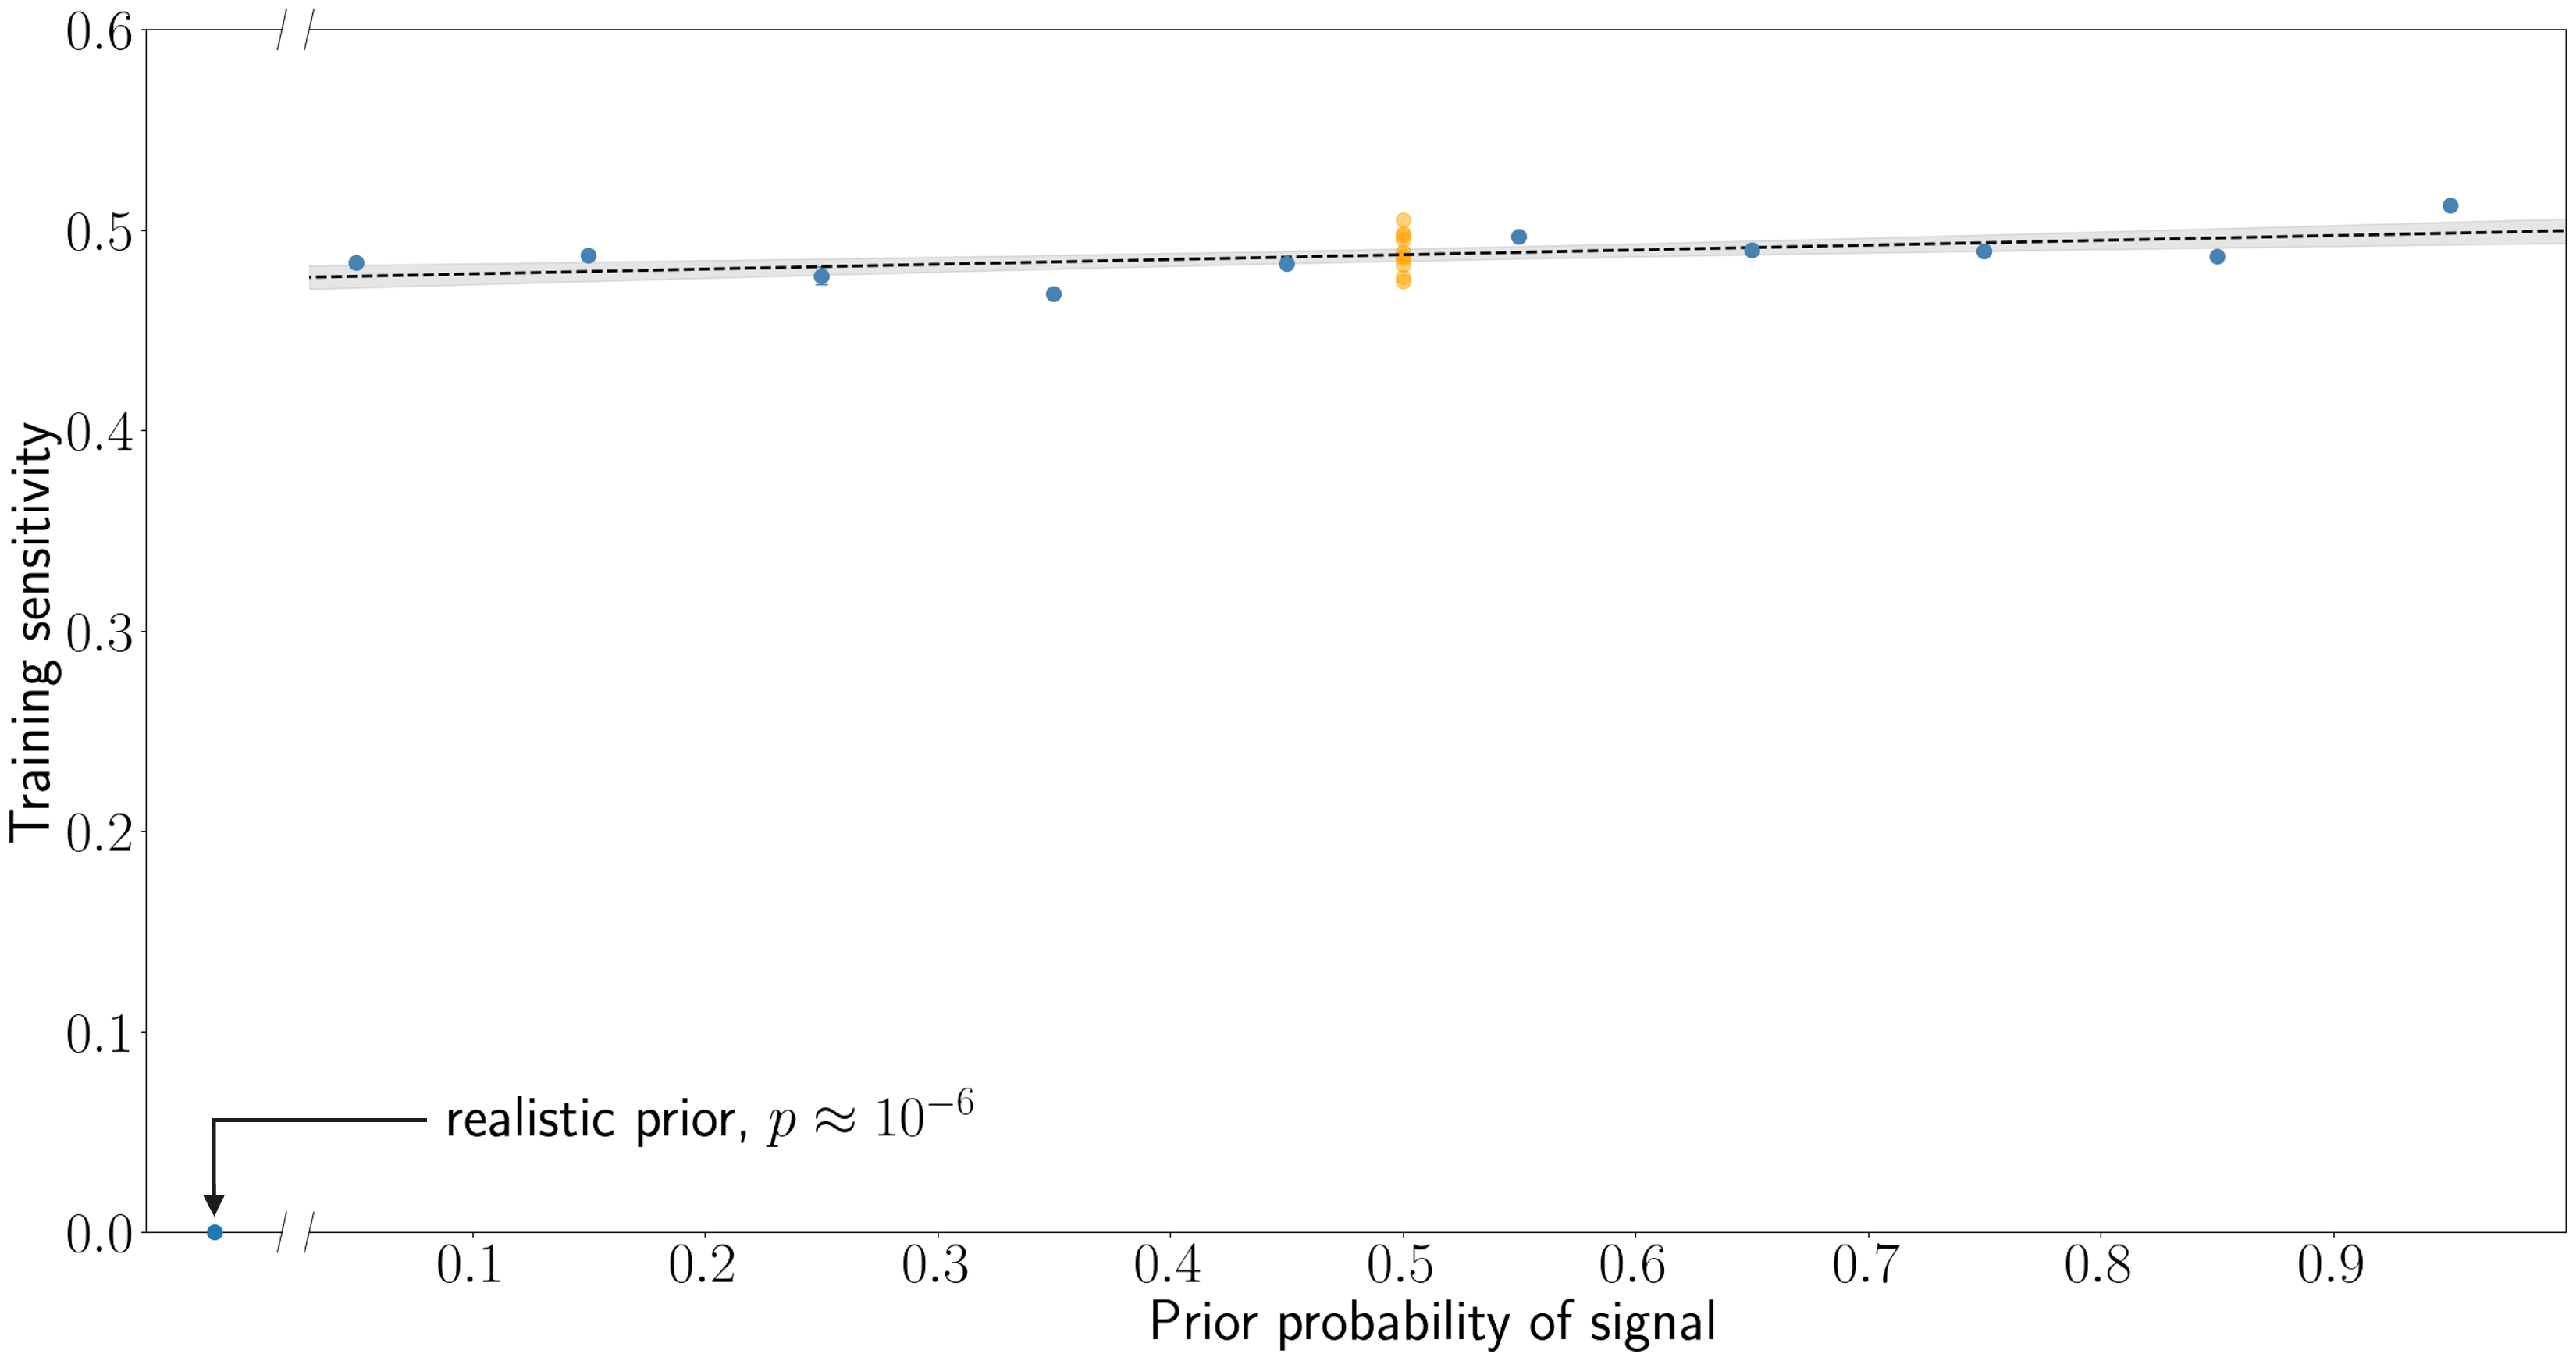
\includegraphics[width=1\textwidth]{./plots/prior_discussion}
	\caption{A very faint positive slope ($m = 0.02\pm0.01$) is observed when relating prior probability to trigger sensitivity (blue dots) of an example 
	convolutional neural network. This could however be attributed to statistical fluctuations in the training fit. An ensemble of networks with the same 
	architecture trained on the same data and with a single prior shows a comparable spread (orange dots).}
	\label{fig:prior-discussion}
\end{figure}

\subsubsection{Filtering \& Downsampling}
\label{sssec:filtering-and-downsampling}

Classical triggers are run in compatibility mode, where 3 UUB bins (\SI{8.3}{\nano\second}) are filtered and downsampled to resemble a single UB bin 
(\SI{25}{\nano\second}). Some information about the trace shape is lost in the process. Logically, a neural network should be able to identify original UUB signal 
traces with more ease than their filtered and downsampled counterparts. Ideal triggers should therefore have a higher efficiency when tested on full bandwidth 
traces

This does not render compatibility mode completely uninteresting for analysis. An effective way of minimizing the trainable parameters in a neural network is 
reducing its' number of input parameters. Filtering and dowmsampling encodes - albeit imperfectly - the input data and reduces the dimensionality by a factor of 
three. This is done in such a way that the UB-like trace contains trace information from a time window that is three times as long for a given number of bins.

Consequently, by filtering and downsampling input data it becomes possible to hand the classifiers additional information while keeping the network size at a fixed
level. The effects this has on predictive power of neural networks is further discussed in \autoref{sec:cnn-performance}. 

\subsection{Choice of labelling}
\label{ssec:choice-of-labelling}

\todo{Muon cut}
\todo{integr. charge cut}

\subsection{Further hyperparameters}
\label{ssec:further-hyperparameters}

\todo{Loss function weighting}
\todo{Loss function background rate pull term}

\section{Convolutional neural networks}
\label{sec:cnn-performance}

\subsection{Architecture}
\label{ssec:cnn-architecture}

\begin{itemize}
	\item Conv2d layer to pool information from 3 PMTs
	\item Conv1d layer to pick up on trace shape
	\item Dense layer to reduce to binary output choice
\end{itemize}

\todo{plot of architecture?}

\subsection{Input size}
\label{ssec:input-size}

\begin{itemize}
	\item Larger input size positively influences efficiency, same SNR level though
\end{itemize}

\todo{signal-to-noise-ratio plot for the same cut values}
\begin{figure}
	\centering
	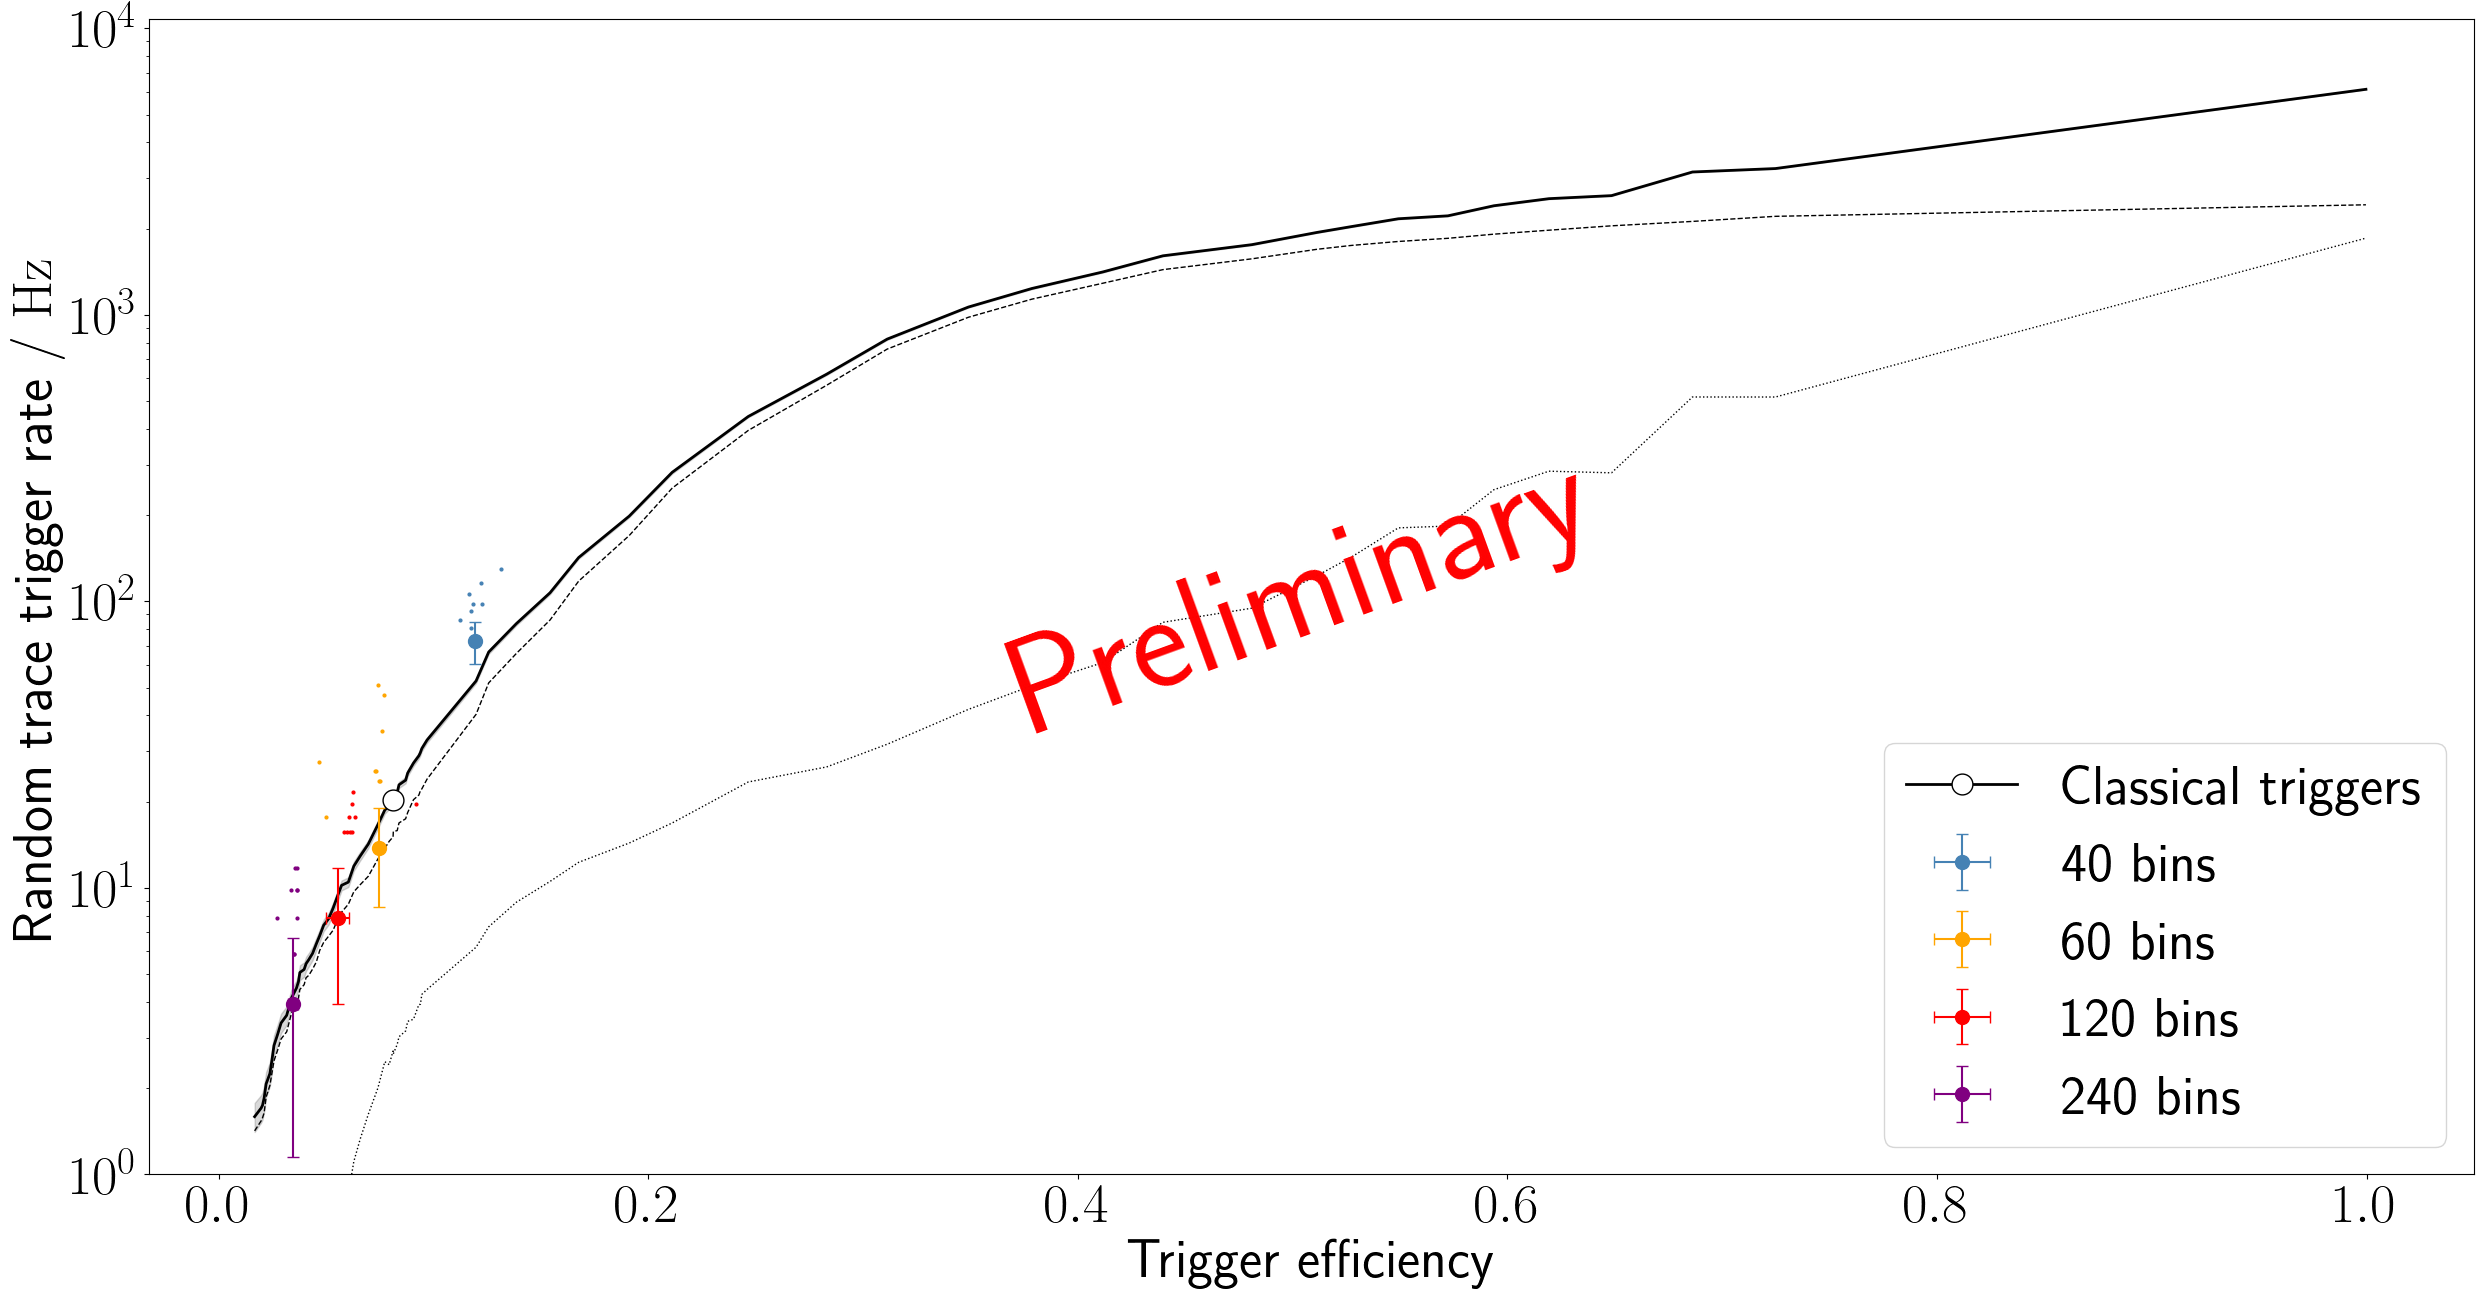
\includegraphics[width=1\textwidth]{./plots/prelim/input_size.png}
	\caption{Input size vs. observed operation parameters}
\end{figure}

\subsection{Kernel size}
\label{ssec:kernel-size}

\begin{itemize}
	\item Larger kernel positively influence efficiency, same SNR level though
\end{itemize}

\todo{signal-to-noise-ratio plot}
\begin{figure}
	\centering
	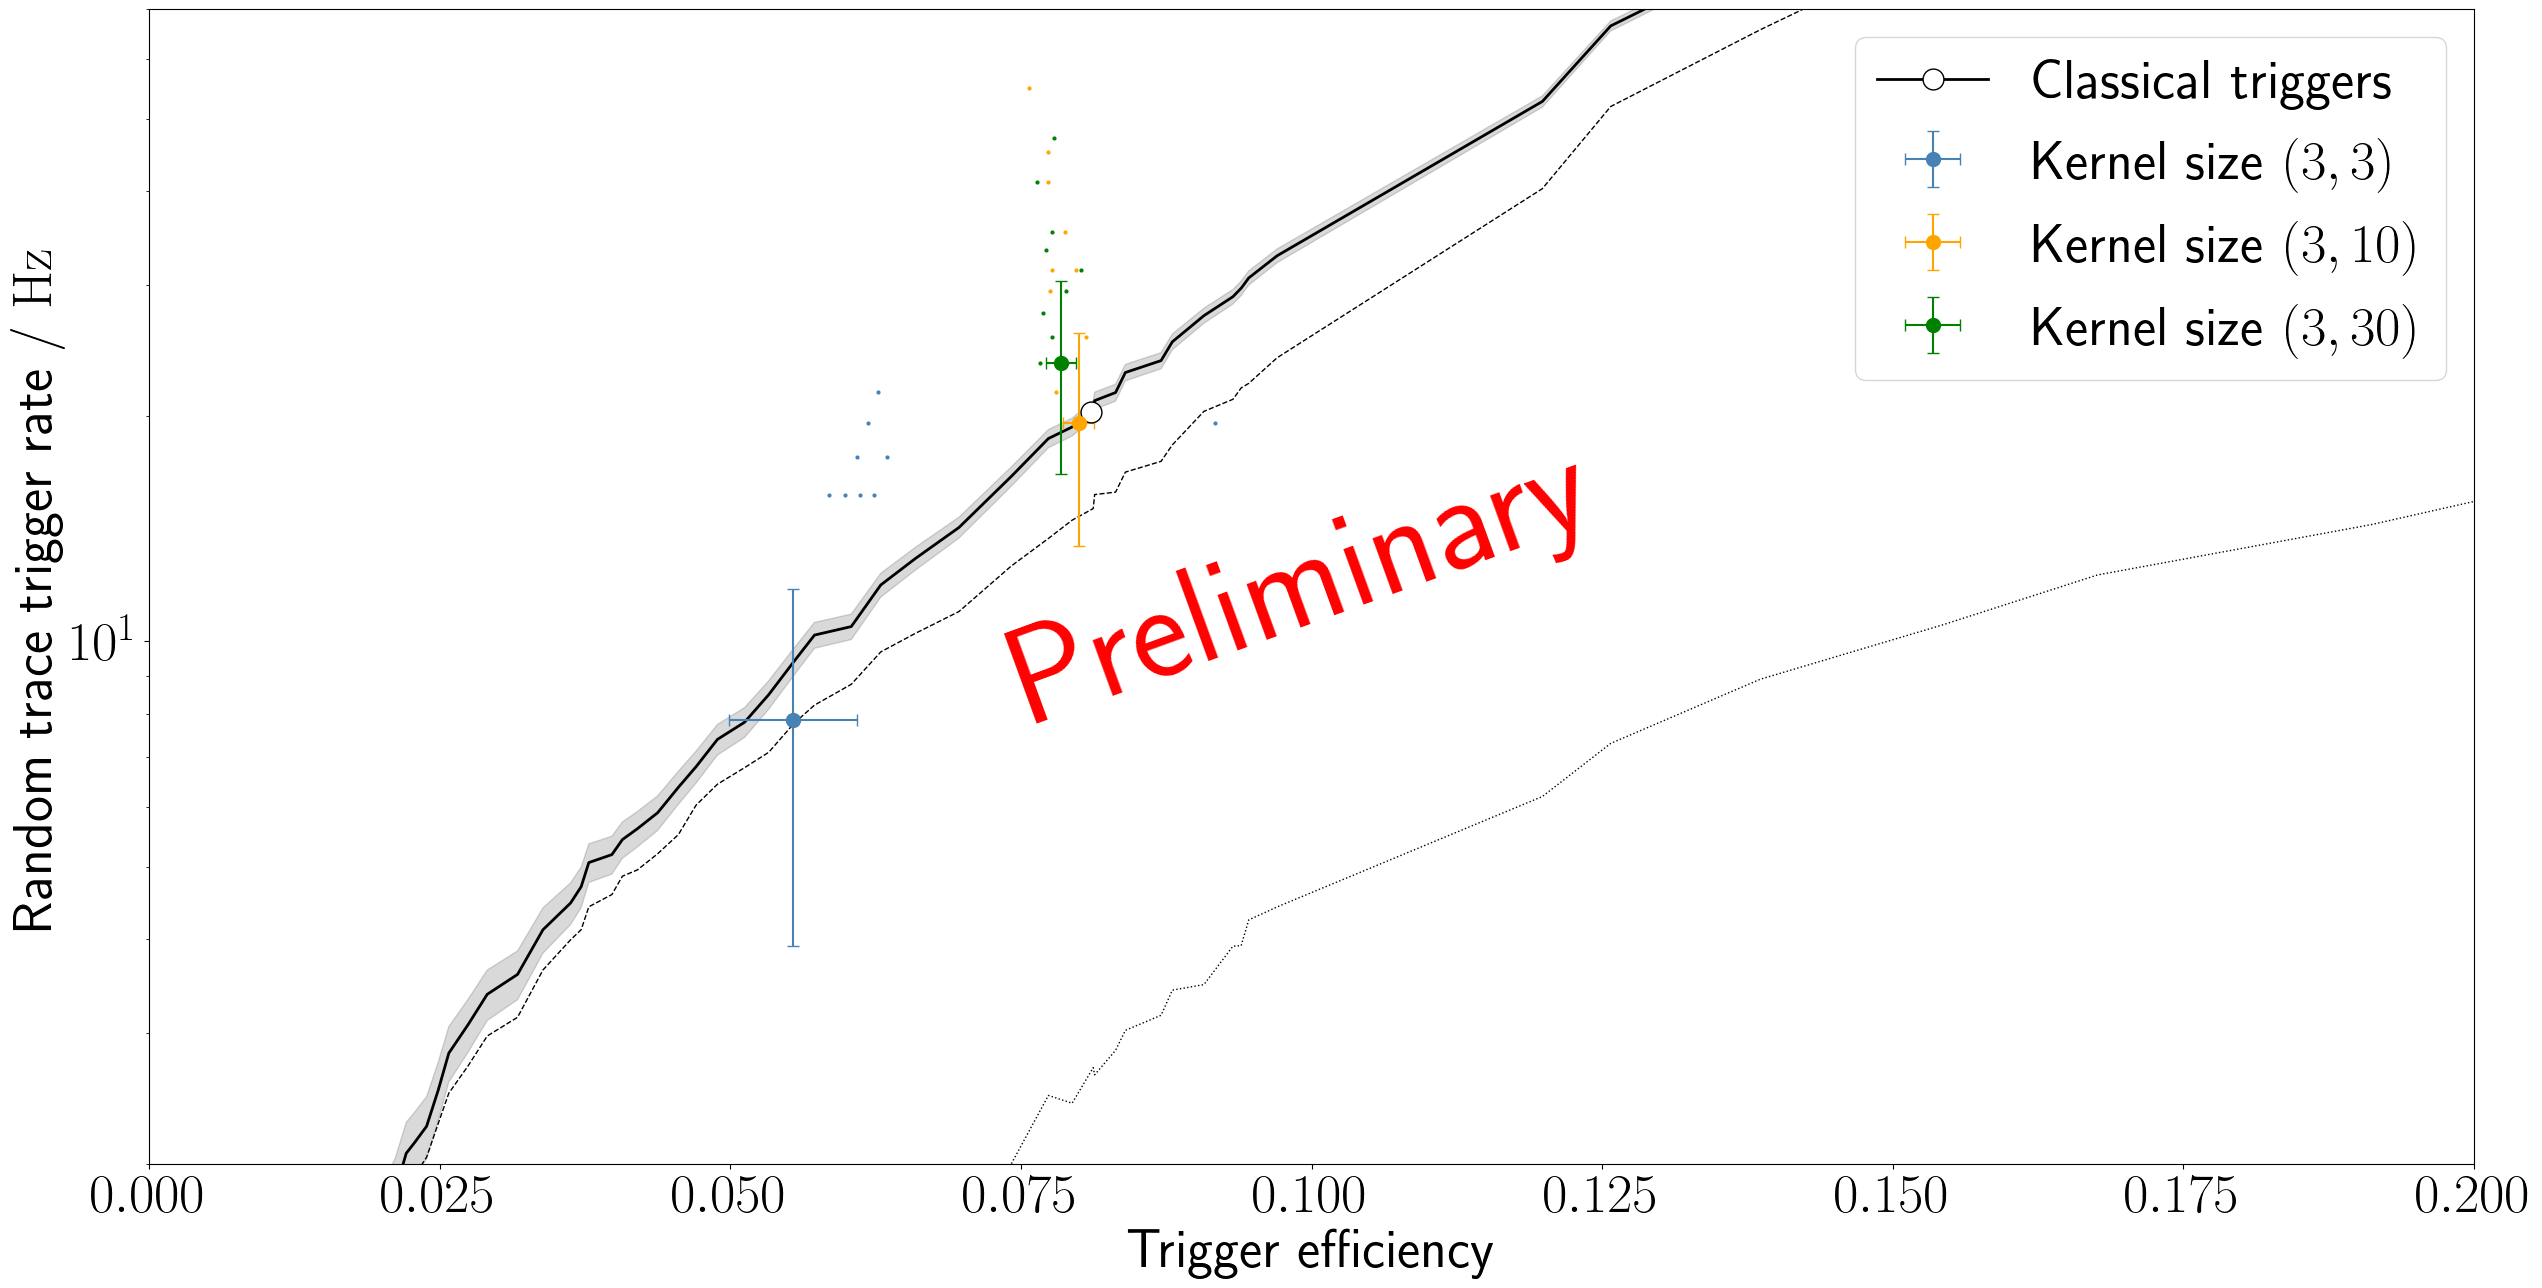
\includegraphics[width=1\textwidth]{./plots/prelim/kernel_size.png}
	\caption{Convolutional kernel size vs. observed operation parameters}
\end{figure}

\subsection{Muon cut}
\label{ssec:muon-cut}

\begin{itemize}
	\item Muons not a viable hyperparameter for network training
	\item Does not decrease trigger rate by sufficient amount
	\item Networks don't converge reproducibly
\end{itemize}

\todo{signal-to-noise-ratio plot}
\begin{figure}
	\centering
	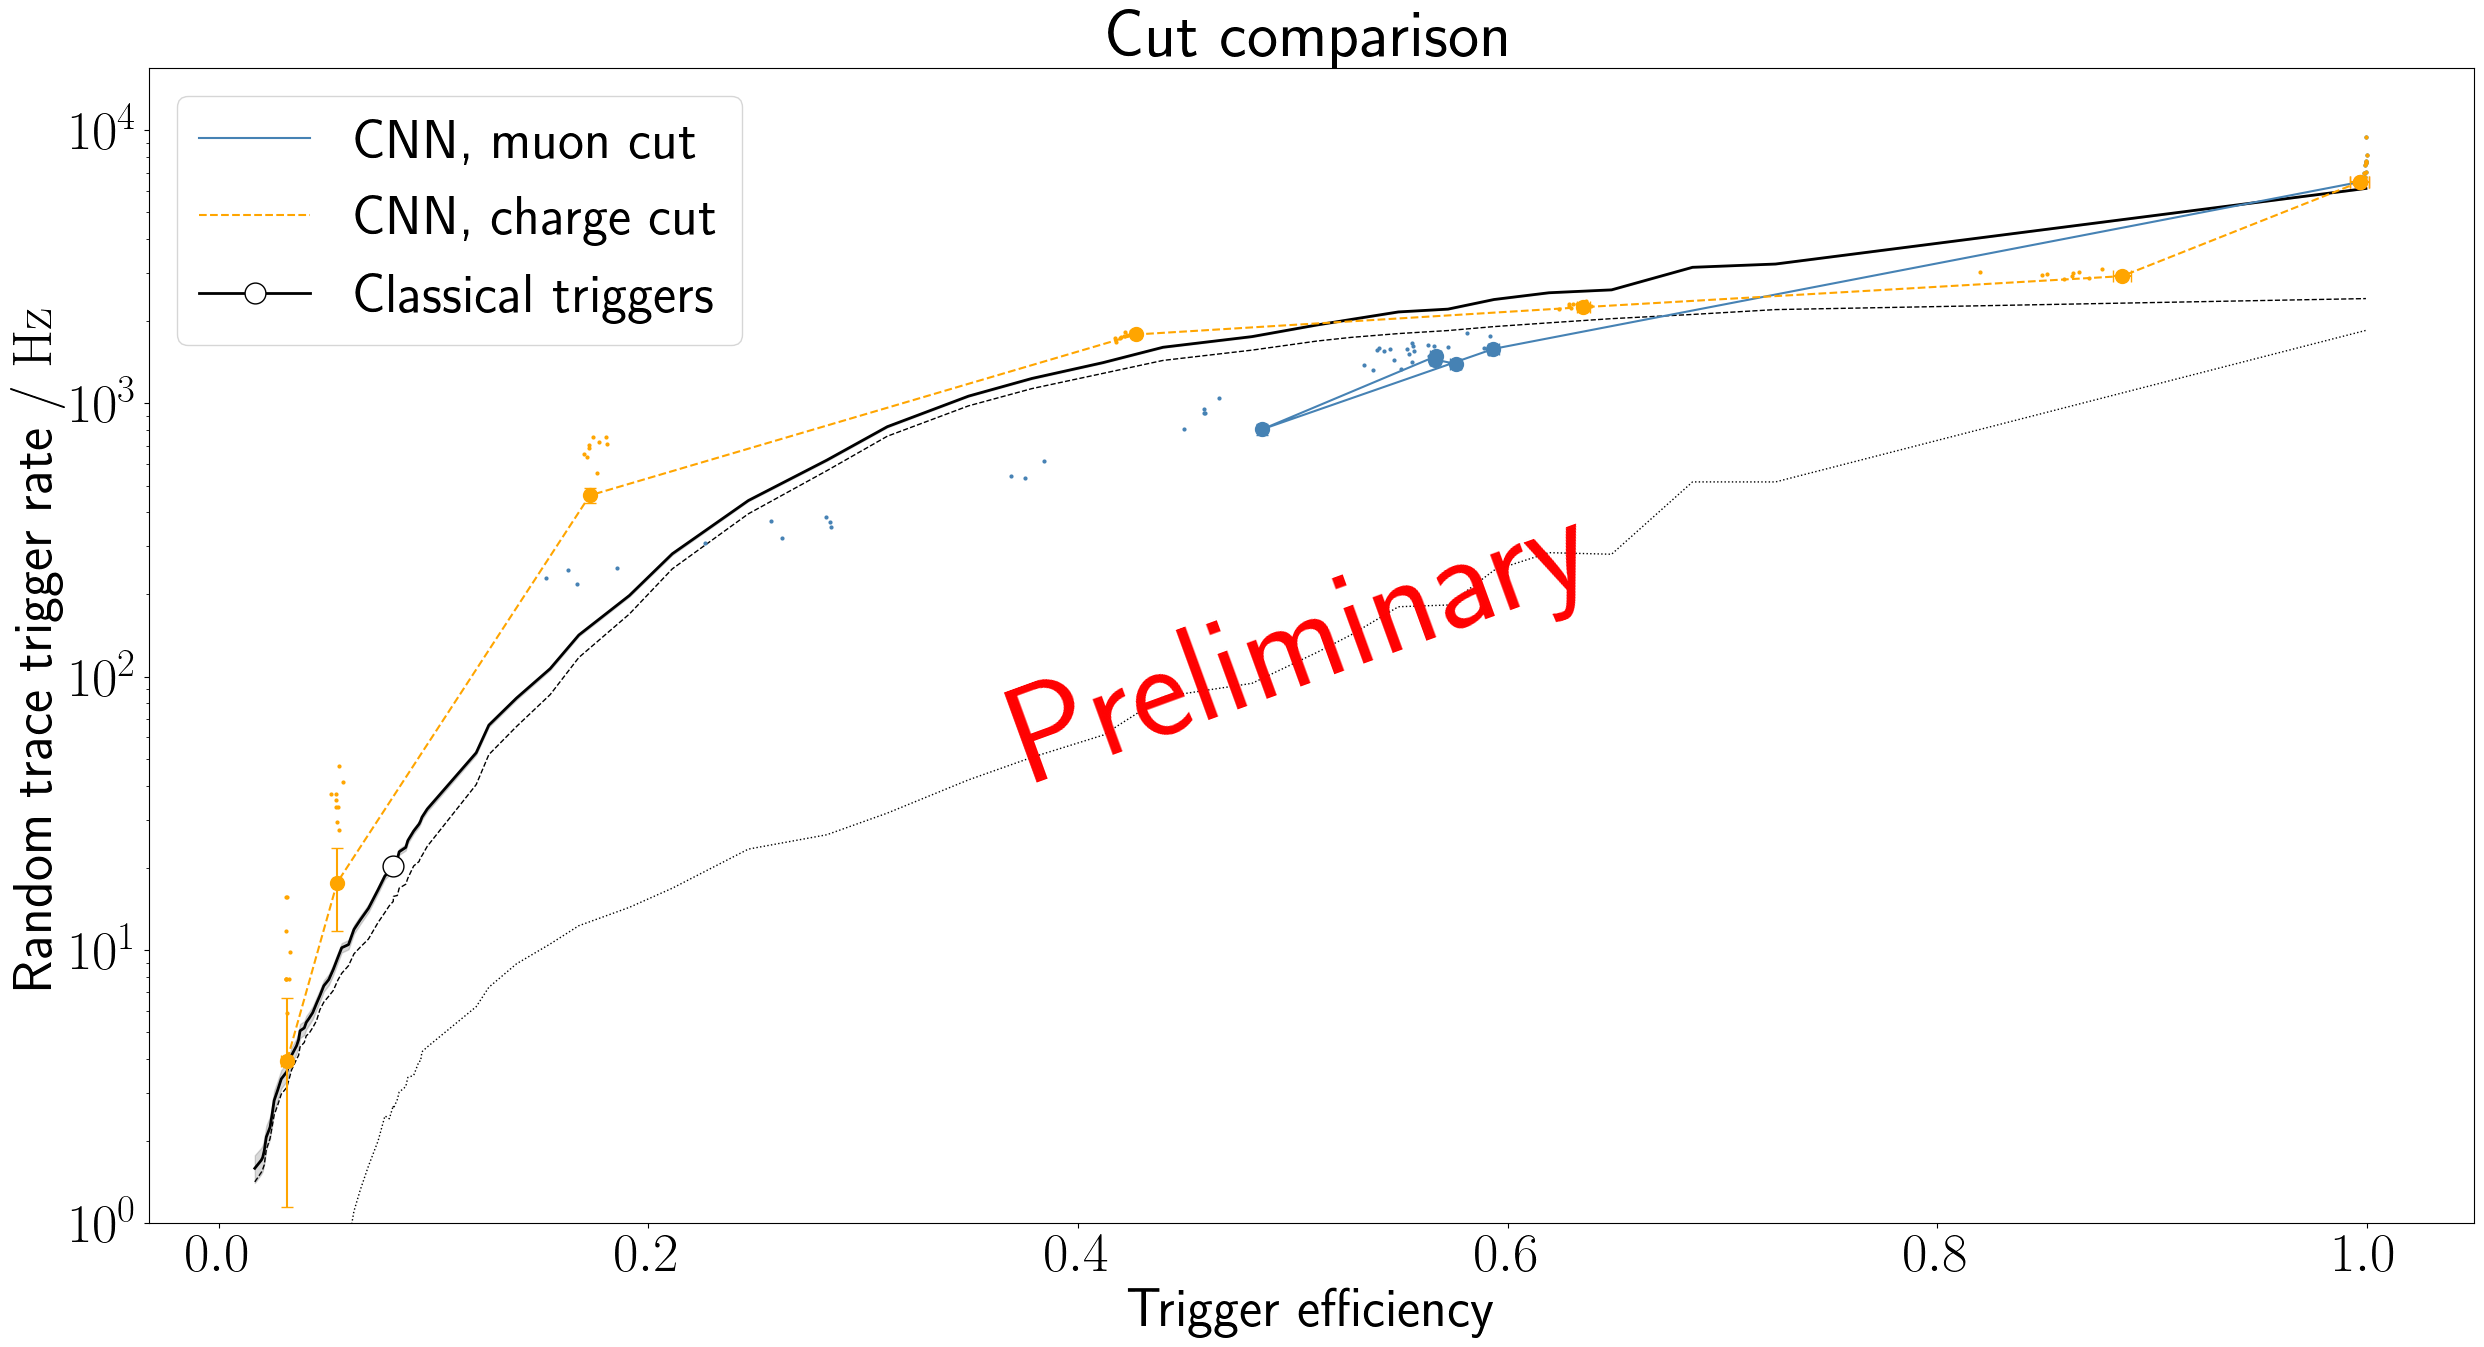
\includegraphics[width=1\textwidth]{./plots/prelim/cut_comparison.png}
	\caption{comparison between muon cut and charge cut}
\end{figure}

\subsection{Charge cut}
\label{ssec:cnn-charge-cut}

\begin{itemize}
	\item Works well with data at hand
	\item offers finer (infinite) resolution in setting cut threshold
\end{itemize}

\todo{signal-to-noise-ratio plot}
\todo{discuss filtering \& downsampling here?}
\todo{signal efficiency ratio}
\begin{figure}
	\centering
	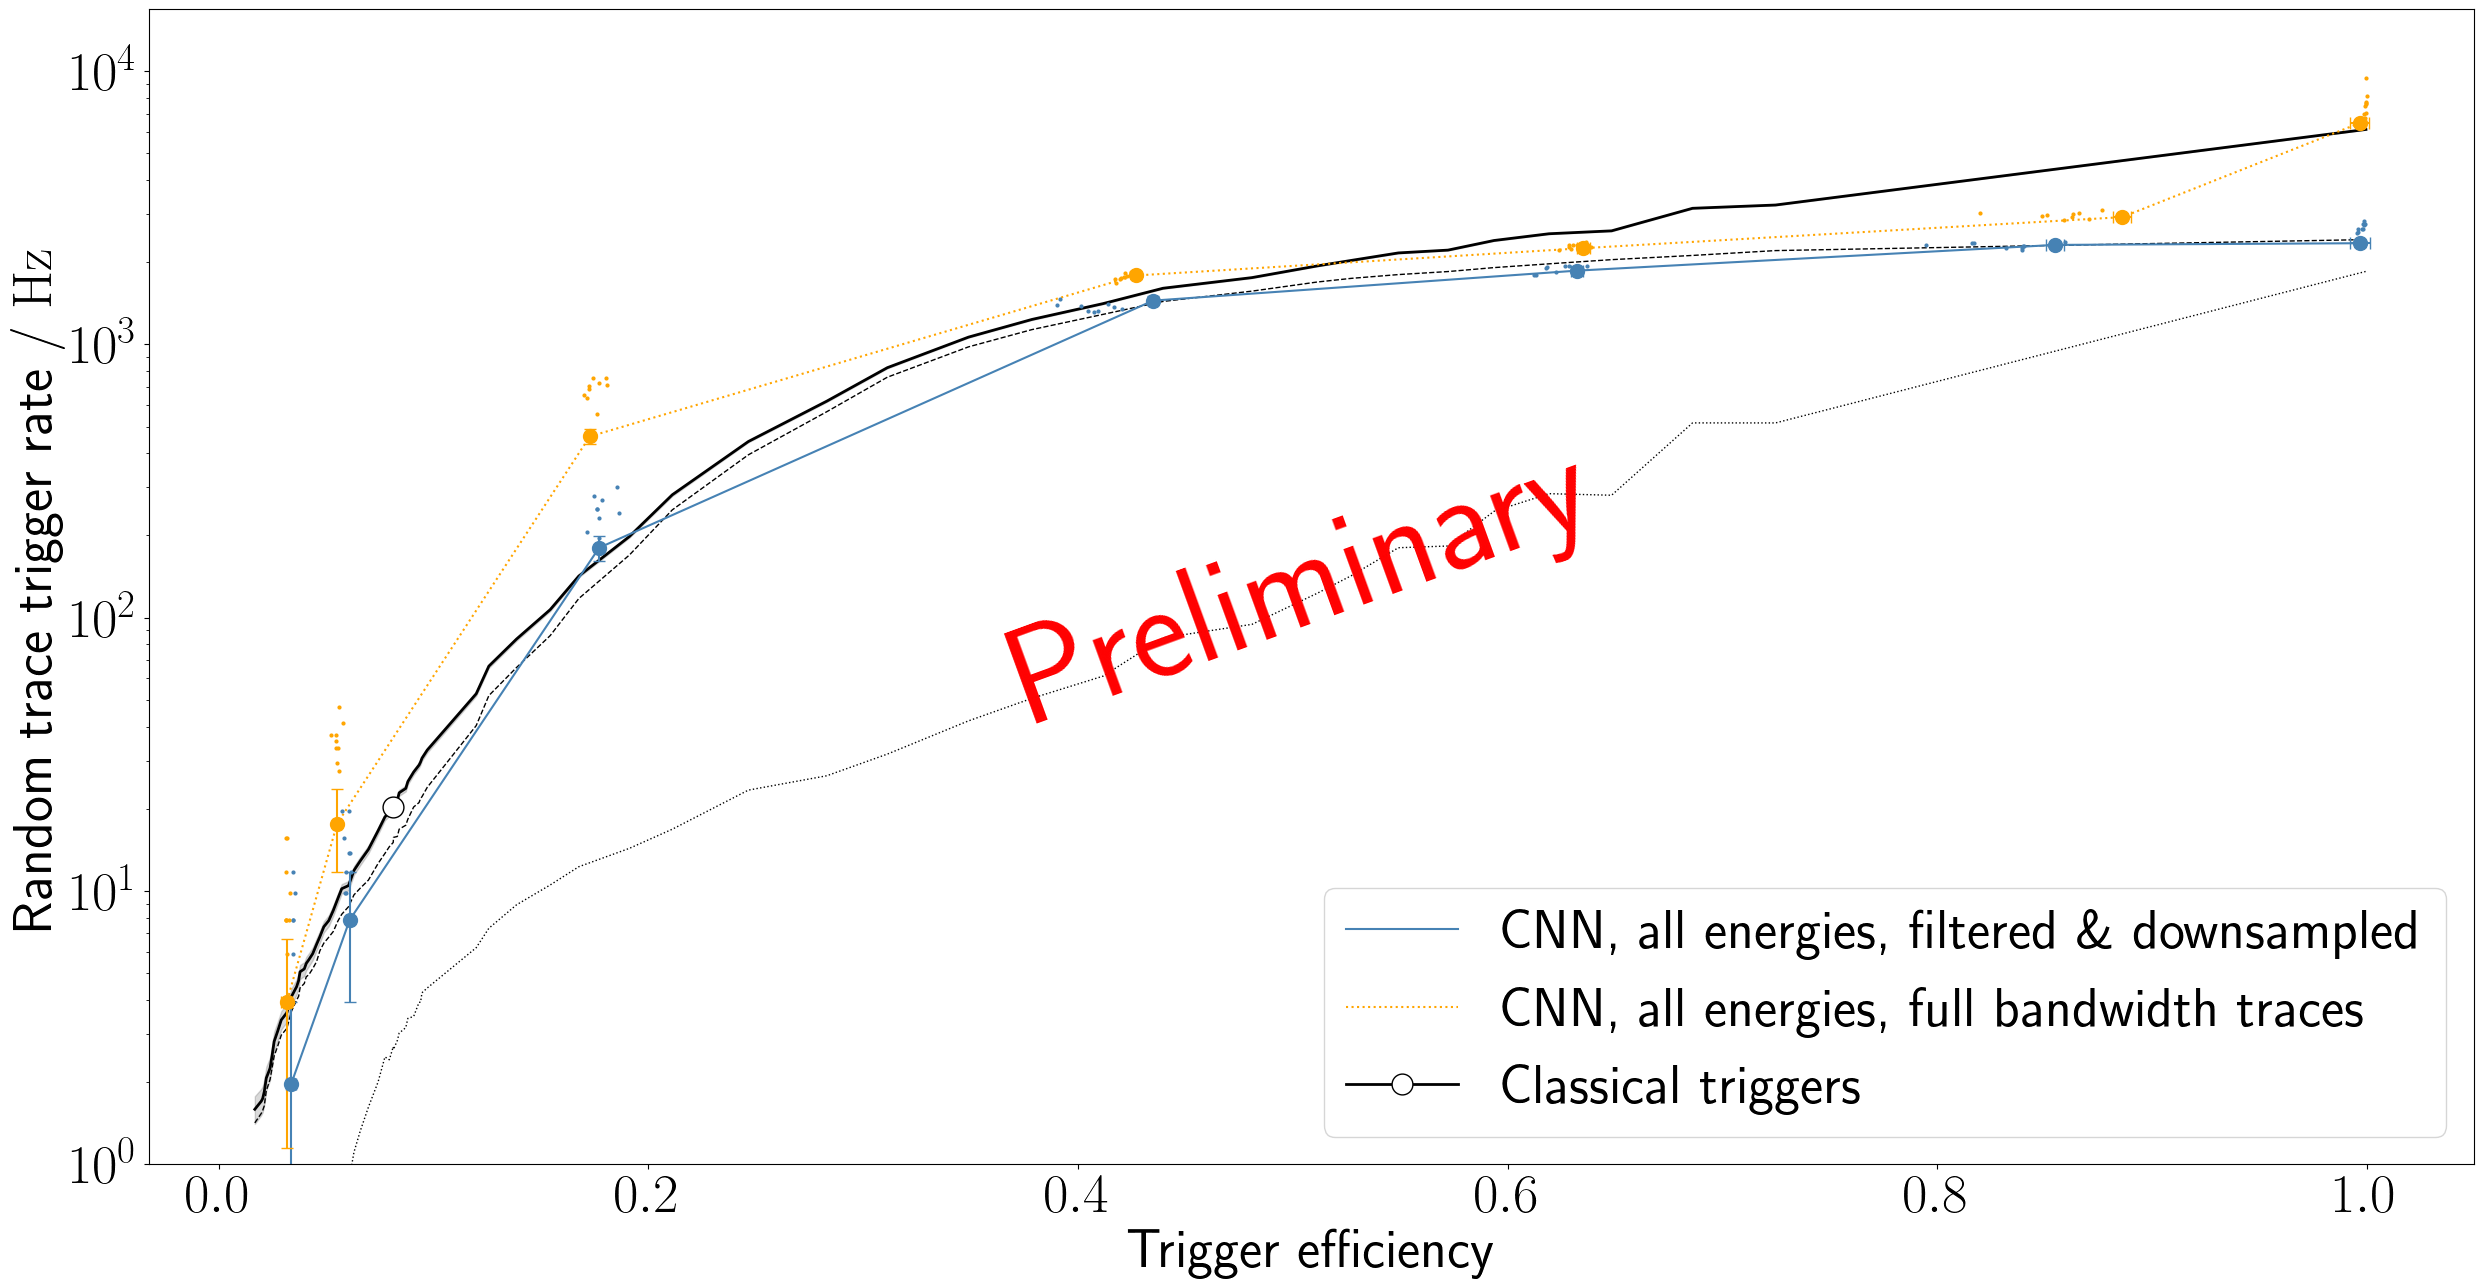
\includegraphics[width=1\textwidth]{./plots/prelim/charge_cut.png}
	\caption{charge cut for full bandwidth and filtered \& downsampled input data}
\end{figure}

\section{LSTM}
\label{sec:lstm-performance}

\subsection{Architecture}
\label{ssec:lstm-architecture}

\begin{itemize}
	\item Discuss choice of architecture
	\item Discuss possibility of using a single layer (instead of 3)
\end{itemize}

\subsection{Charge cut}
\label{ssec:cnn-charge-cut}

\todo{signal-to-noise-ratio plot}
\begin{figure}
	\centering
	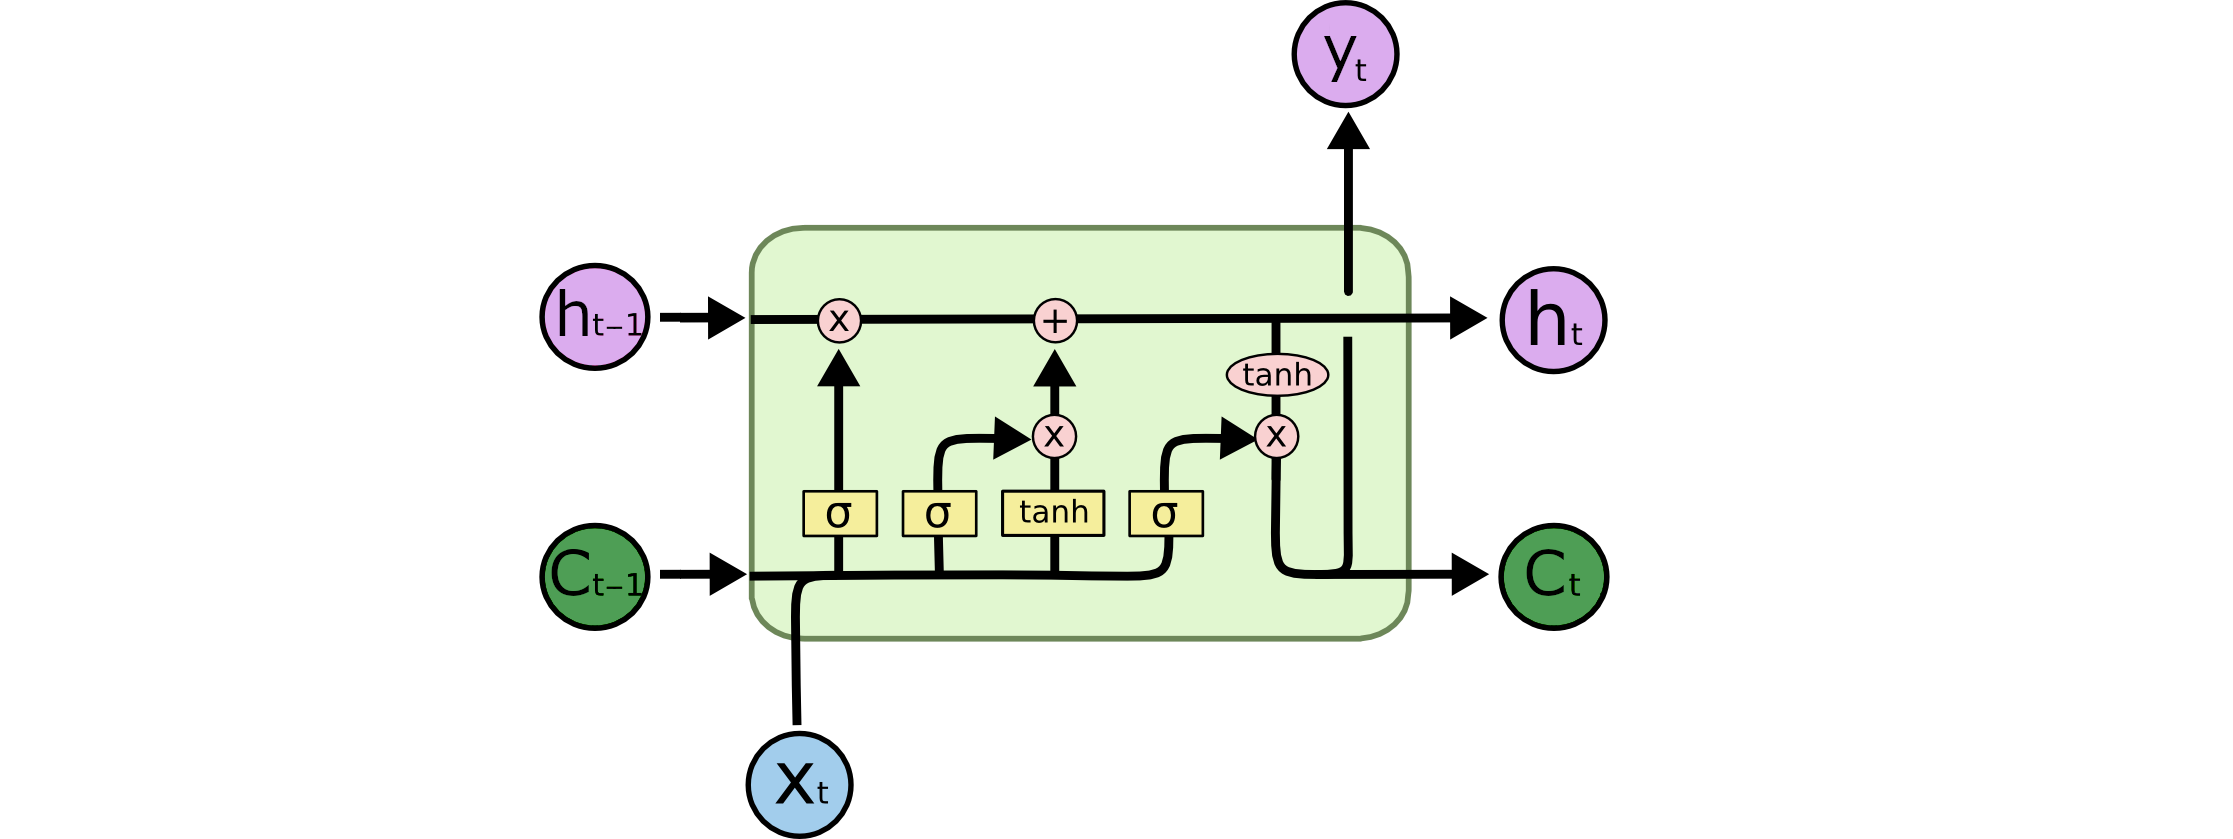
\includegraphics[width=1\textwidth]{./plots/prelim/LSTM.png}
	\caption{performance of LSTM}
\end{figure}